\section{Accelerated compute: GPUs and the AI workload path}
\label{sec:accelerated-compute}

An accelerator is not a fungible resource the way a CPU core or a gigabyte of RAM is: a GPU is
either present on a physical host or it is not, and whatever isolates one tenant's use of it from
another's is either enforced by the device driver and the orchestrator or it is not enforced at
all. This section asks two narrow questions about what \Flux actually ships today. First, what does
``pluggable GPU'' mean in code — is a GPU attached to a workload as a whole device, a slice of a
device, or something attachable and detachable at runtime? Second, what is the isolation boundary
between two tenants placed on the same machine? The answers are more restrictive than the roadmap's
language suggests, and one of the mechanisms below has a correctness defect worth stating plainly
rather than filing as a performance footnote. The evidence surveyed spans four repositories:
\texttt{fluxai} and \texttt{fluxai-\allowbreak{}enterprise} (an inference-as-a-service product), \texttt{pouwbackend}
(the \FluxEdge compute-rental marketplace), and \texttt{fluxai-\allowbreak{}fluxedge} (the GitOps glue between the
first two).

\subsection{GPU allocation as implemented}
\label{sec:accelerated-compute-allocation}

On the \FluxEdge marketplace, a rented workload's container requests a GPU the same way any
Kubernetes workload does: a resource quantity under the vendor device-plugin key \texttt{nvidia.com/gpu}
in the pod's \texttt{resources.\allowbreak{}limits}\slash\texttt{requests} \shipped\ \srccode{pouwbackend/\allowbreak{}rancher/\allowbreak{}deployment.go}{2155-2163}.
\texttt{set\allowbreak{}Resource\allowbreak{}Limit} reconciles the requested GPU \emph{count} against the rented computer's
actual GPU inventory, walking a bus-indexed enumeration of the machine's physical devices
(\texttt{newGPUIndexer}, NVIDIA-relative indexing) and appending each chosen bus index to the set of
GPUs already consumed by earlier containers of the same deployment \shipped\ \srccode{pouwbackend/\allowbreak{}rancher/\allowbreak{}deployment.go}{914-982},
\srccode{pouwbackend/\allowbreak{}rancher/\allowbreak{}deployment.go}{1245-1270}. Isolation between deployments sharing a rented
computer --- which on \FluxEdge belong to one renter, since a computer is rented exclusively
\srccode{pouwbackend/\allowbreak{}models/\allowbreak{}market\_place.sql.go}{1182-1190} --- is
then a single mechanism: the chosen bus indices are written into the container's
\texttt{NVIDIA\_VISIBLE\_DEVICES} environment variable \shipped\ \srccode{pouwbackend/\allowbreak{}rancher/\allowbreak{}deployment.go}{967-971}.
There is no further Flux-specific sandboxing layered on top of this; the isolation guarantee is
whatever the Kubernetes NVIDIA device plugin and the container runtime provide for an
environment-variable-scoped device list.

No time-slicing, no NVIDIA Multi-Instance GPU (MIG) partitioning, and no virtual-GPU (vGPU)
mechanism exists anywhere in the four repositories surveyed \shipped\ \srccode{pouwbackend/\allowbreak{}rancher/\allowbreak{}deployment.go}{914-982}.
This is a coherent design choice, not an oversight: whole-device passthrough with
environment-variable isolation is simple to reason about and gives strong isolation — a device
cannot be double-assigned across pods on the same node, because the device plugin never advertises
more \texttt{nvidia.com/gpu} resources than there are physical devices. The consequence is equally
direct: the granularity of what can be sold is fixed at one physical GPU. \FluxEdge cannot today
offer a fractional share of a GPU to two tenants concurrently; the only way to approximate a smaller
unit of accelerated compute is to dedicate an entire device to one renter and price accordingly.

\subsection{The contention defect: a resource request that disappears}
\label{sec:accelerated-compute-contention}

If none of a container's requested GPUs can be assigned --- the computer reports no NVIDIA
device, or every device is already taken by an earlier container of the same deployment ---
\texttt{set\allowbreak{}Resource\allowbreak{}Limit} does not reject the request and does not queue it for a computer with
sufficient capacity. It deletes the \texttt{nvidia.com/gpu} key from both \texttt{Limits} and
\texttt{Requests} on the container spec entirely \shipped\ \srccode{pouwbackend/\allowbreak{}rancher/\allowbreak{}deployment.go}{972-975}.
The workload is then scheduled and runs CPU-only, with no accelerator, and with no error surfaced to
the caller from this code path; the only trace is a log line from a failed resource-consumption
write, which is itself only logged rather than propagated \shipped\ \srccode{pouwbackend/\allowbreak{}rancher/\allowbreak{}deployment.go}{978-980}.
If only some of the requested GPUs can be assigned, the container receives that subset in
\texttt{NVIDIA\_VISIBLE\_DEVICES} while its declared limit is left unchanged, again with no error
\shipped\ \srccode{pouwbackend/\allowbreak{}rancher/\allowbreak{}deployment.go}{950-968}.

This is a correctness defect, not a performance characteristic. A caller who pays for and requests a
GPU-bearing deployment can receive a deployment silently missing the one resource that made the
request meaningful, and nothing in the API response distinguishes that outcome from a fully
provisioned rental. The correct behaviour, on contention, is to reject the rental request outright
or to queue it until a matching computer becomes available — either choice preserves the invariant
that a caller can trust an accepted request to mean what it says. Silently stripping the resource
line instead breaks that invariant in a way a paper describing this system should not pass over.

\subsection{``Pluggable'' or hot-attachable GPU: no code, no exception}
\label{sec:accelerated-compute-pluggable}

The roadmap's language of a ``pluggable'' or hot-attachable GPU has no counterpart in any of the
four repositories surveyed \srcdoc{plan/conflicts.md, C23}. An exhaustive search across all four
repositories for hot-attach, hot-plug, hot-swap, and pluggable terminology returns exactly one hit
outside vendor code, and it is unrelated: a \texttt{HotSwap} boolean field on OVH's public cloud
catalog API describing disk RAID hot-swap on dedicated servers, not GPU attachment
\srccode{pouwbackend/\allowbreak{}premium/\allowbreak{}ovh/\allowbreak{}ovh.go}{320}. There is no code anywhere in \texttt{fluxai},
\texttt{fluxai-\allowbreak{}enterprise}, \texttt{fluxai-\allowbreak{}fluxedge}, or \texttt{pouwbackend} that attaches a GPU to
an already-running container, or that reallocates a GPU between tenants without a pod
restart or reschedule. This is tagged \vision: it names a capability the roadmap gestures toward
that does not exist in code today, and the paper does not speculate about what a future
implementation might look like beyond that.

\subsection{Two product surfaces, easy to conflate}
\label{sec:accelerated-compute-surfaces}

The corpus contains two separate GPU-bearing product surfaces, and describing either as if it were
the other would misstate the system.

\texttt{fluxai} and \texttt{fluxai-\allowbreak{}enterprise} are an inference-as-a-service product — chat
completions, image generation, document intelligence — backed by a fixed, admin-provisioned pool of
GPU servers internally called ``RGP'' (Remote GPU). An administrator creates an RGP record, selects a
model, and triggers an asynchronous Ansible playbook that connects over SSH and stands up the
inference stack on the target rig \shipped\ \srccode{fluxai/\allowbreak{}fluxai\_admin/\allowbreak{}pages/\allowbreak{}views\_rgp.py}{36,468}.
There is no self-service provisioning path for an external caller in this product; capacity changes
only through this admin workflow, and \texttt{fluxai} is itself a tenant application deployed onto
\FluxCloud rather than part of the cloud substrate.

\texttt{pouwbackend} is the backend of \FluxEdge, a separate, Rancher/Kubernetes-orchestrated
compute-rental marketplace with its own OpenAPI-documented REST interface and its own CLI
\shipped\ \srccode{pouwbackend/\allowbreak{}rest\_api/\allowbreak{}v1/\allowbreak{}openapi.yaml}{1-4}. This is the mechanism described in
\S\ref{sec:accelerated-compute-allocation}--\S\ref{sec:accelerated-compute-contention}.

\texttt{fluxai-\allowbreak{}fluxedge} is the GitOps glue between the two: a repository of Kubernetes manifests and
Argo \texttt{Workflow} templates that clone the repository, build a \texttt{kustomize} overlay for a
given model, and \texttt{kubectl apply} it onto a node selected at submission time by \FluxEdge
\shipped\ \srccode{fluxai-fluxedge/\allowbreak{}custom-workflow-fluxone.yaml}{7-9,21-52}. In other words,
\texttt{fluxai}'s own inference pods are themselves provisioned as workloads on \FluxEdge — the two
product surfaces are physically coupled by self-hosting even though their APIs are independent
products, and a reader should not assume that describing one describes the other.

\begin{figure}[H]
\centering
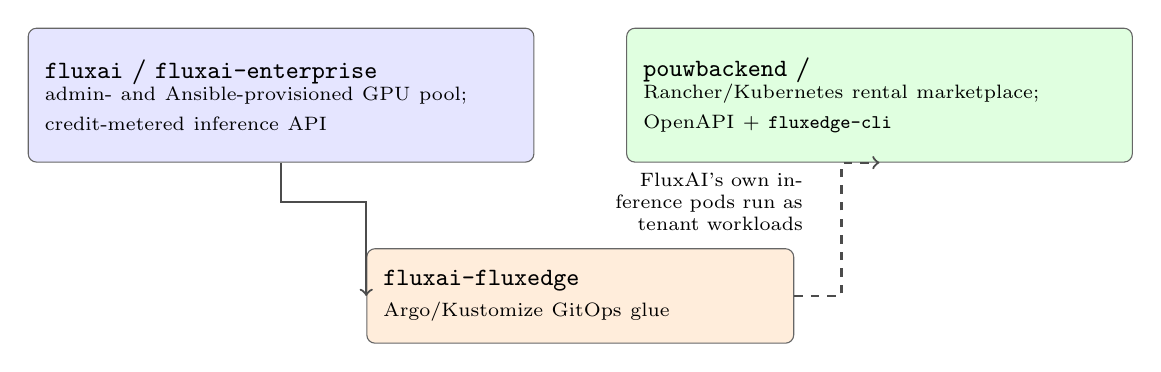
\begin{tikzpicture}[font=\small,
  b/.style={draw=black!60, rounded corners=3pt, align=left, inner sep=6pt, text width=6.0cm,
            minimum height=1.7cm},
  ai/.style ={b, fill=blue!10},
  edge/.style={b, fill=green!12},
  glue/.style={b, fill=orange!14, text width=5.0cm, minimum height=1.2cm},
]
\node[ai]   (ai)   at (0,3.1)  {\textbf{\texttt{fluxai} / \texttt{fluxai-\allowbreak{}enterprise}}\\
  {\scriptsize admin- and Ansible-provisioned GPU pool;\\credit-metered inference API}};
\node[edge] (fe)   at (7.6,3.1) {\textbf{\texttt{pouwbackend} / \FluxEdge{}}\\
  {\scriptsize Rancher/Kubernetes rental marketplace;\\OpenAPI ${+}$ \texttt{fluxedge-cli}}};
\node[glue] (glue) at (3.8,0.55) {\textbf{\texttt{fluxai-\allowbreak{}fluxedge}}\\
  {\scriptsize Argo/Kustomize GitOps glue}};

\draw[->, thick, black!70] (ai.south) -- ++(0,-0.5) -| (glue.west);
\draw[->, thick, dashed, black!70] (glue.east) -- ++(0.6,0) |- (fe.south);
%% Standalone, in the gap between the two boxes: on the edge at pos=0.72 it
%% printed on top of the pouwbackend/FluxEdge box.
\node[font=\scriptsize, text width=3.3cm, align=right, anchor=east] at (6.75,1.75)
  {FluxAI's own inference pods run as \FluxEdge{} tenant workloads};
\end{tikzpicture}
\caption{The two GPU-bearing product surfaces and the self-hosting relationship between them.}
\label{fig:accelerated-compute-surfaces}
\end{figure}

\subsection{A module name that is not a mechanism}
\label{sec:accelerated-compute-pouw}

\texttt{pouwbackend} is a mature compute-rental marketplace, and the paper describes it as exactly
that. Despite the name, ``Proof of Useful Work'' is not a designed consensus or verification
mechanism anywhere in this code. The only in-code hits for the term are a GPU mining-overclock
preset applied to a rig when its rental ends \shipped\ \srccode{pouwbackend/\allowbreak{}grpc\_server/\allowbreak{}market\_place/\allowbreak{}computer.go}{502,517},
and a Postgres schema documentation file that self-describes the database as the ``flux Prove Of
Useful Work Database (POUW)'' — branding, not a mechanism \shipped\ \srccode{pouwbackend/\allowbreak{}sql/\allowbreak{}.tbls.yml}{3}.
There is no submit-work, verify-work, or reward-work RPC triple; no on-chain anchoring of compute
results; and no linkage of any kind to \fluxd consensus. ``PoUW'' survives in this codebase only as a
Go module path and a database nickname. The paper does not describe \Flux as having a
proof-of-useful-work mechanism anywhere, and this section is where that is stated once, plainly, for
the record.

\subsection{The machine-facing surface: scoped tokens, forward to \S18}
\label{sec:accelerated-compute-machine-facing}

The \FluxEdge REST interface — OpenAPI 3.1.1, base path \texttt{/api/v1} — and its accompanying CLI,
\texttt{fluxedge-cli}, are the machine-facing surface this paper's agent-provisioning discussion in
\S18 depends on, not the fixed-credit inference API described above \shipped\ \srccode{pouwbackend/\allowbreak{}rest\_api/\allowbreak{}v1/\allowbreak{}openapi.yaml}{1-4}.
Authentication is by bearer token, and a key's privileges are enumerated rather than all-or-nothing:
\texttt{start\_rental}, \texttt{stop\_rental}, \texttt{start\_deployment}, \texttt{stop\_deployment},
and \texttt{get\_balance} \shipped\ \srccode{pouwbackend/\allowbreak{}rest\_api/\allowbreak{}v1/\allowbreak{}openapi.yaml}{2576-2581},
enforced in code by mapping each rental and deployment endpoint path to its required privilege
string --- the balance privilege is documented but has no entry in that map
\shipped\ \srccode{pouwbackend/\allowbreak{}rest\_api/\allowbreak{}ratelimit.go}{375-390}. Requests are rate-limited to two per
second per key and two per second per source IP \shipped\ \srccode{pouwbackend/\allowbreak{}rest\_api/\allowbreak{}ratelimit.go}{41-42};
a key or IP that accumulates five rate-limit violations within a five-minute window is automatically
revoked, its owner notified by email, and its cache entry evicted \shipped\ \srccode{pouwbackend/\allowbreak{}rest\_api/\allowbreak{}ratelimit.go}{43-45,203-222}.
This is a bounded, revocable \emph{action} authority — a human operator can mint a key that may start
rentals but not stop them, for example — suitable for handing to an autonomous agent with a defined
blast radius. No MCP server and no Terraform provider exist in any of these four repositories; the
MCP tools that do exist in the \Flux stack live elsewhere and are outside this section's scope, taken
up in \S18.

\subsection{Metering and the overdraft window, forward to \S16}
\label{sec:accelerated-compute-metering}

\texttt{fluxai}'s credit metering is asynchronous and eventually consistent rather than synchronous.
Each request is gated on a positive credit balance at call time, but usage is not deducted
immediately: token consumption accumulates in a Redis cache keyed per user with a 300-second expiry
\shipped\ \srccode{fluxai/\allowbreak{}api/\allowbreak{}cache.py}{9-32}, and a separate scheduled command later scans the
accumulated keys, applies the deduction to the persisted balance inside a locked transaction, and
clears the cache \shipped\ \srccode{fluxai/\allowbreak{}api/\allowbreak{}management/\allowbreak{}commands/\allowbreak{}process\_token\_usage.py}{41-99}.
The 300-second cache window is a real overdraft bound: a caller can spend up to that much usage
before the persisted balance reflects it, and the periodic flush job that closes the window is
itself scheduled through a live database-configured dispatcher rather than a fixed interval fixed in
source \shipped\ \srccode{fluxai/\allowbreak{}setup/\allowbreak{}crons/\allowbreak{}django\_cron}{2}. Any future product that prices
consumption rather than a subscription tier inherits this same window unless it is metered
differently; \S16's discussion of billing accuracy should carry this bound forward rather than
assume synchronous debiting.

\subsection{A gap for agent autonomy: key issuance}
\label{sec:accelerated-compute-key-issuance}

Nothing in \S\ref{sec:accelerated-compute-machine-facing} solves the problem of an agent obtaining
its own credential in the first place. API-key issuance is not exposed anywhere in the documented
REST v1 surface — only consumption is. The API's own quick-start documentation points a caller to the web
dashboard to obtain a key \shipped\ \srccode{pouwbackend/\allowbreak{}rest\_api/\allowbreak{}v1/\allowbreak{}openapi.yaml}{61}. A human must
mint a scoped key through that dashboard before an agent can use the \FluxEdge API autonomously; there
is no REST or CLI self-service path for an agent to request or rotate its own credential. This gap
is exactly the boundary \S17 and \S18 need to address for a fully autonomous provisioning workflow.

\subsection{Natural-language deployment: \texttt{DeploymentYAML}, forward to \S19}
\label{sec:accelerated-compute-nl-deploy}

\texttt{pouwbackend} exposes a gRPC method, \texttt{DeploymentYAML}, that generates Kubernetes YAML
from a natural-language prompt \shipped\ \srccode{pouwbackend/\allowbreak{}grpc\_server/\allowbreak{}market\_place/\allowbreak{}deployment.go}{1784-1812}.
The generation pipeline first performs a vector search over existing marketplace application YAMLs
to build retrieval-augmented context \shipped\ \srccode{pouwbackend/\allowbreak{}ai/\allowbreak{}fluxai.go}{188-191,241-244},
then dispatches a chat-completion request against a pinned model (``Llama 3.1 8B'') or, depending on
configuration, a third-party provider \shipped\ \srccode{pouwbackend/\allowbreak{}ai/\allowbreak{}fluxai.go}{212,266}. This is
the strongest existing evidence in the surveyed corpus for agent-native provisioning: a natural-language
deployment path is not a hypothetical for a future release, a form of it already ships. It is also,
for that reason, the concrete artifact \S19 should hold up when it takes up the question of whether a
generated specification is reviewable before it is signed and run.

\subsection{Resource accounting on the FluxOS side}
\label{sec:accelerated-compute-fluxos}

On the orchestration side, \FluxOS's per-tier resource allowances and its per-application hardware
check both express only the resource vector $\resvec = (\mathrm{cpu}, \mathrm{ram}, \mathrm{hdd})$:
the Cumulus/Nimbus/Stratus tier table gives total and application-available CPU (in tenths of a
core), RAM, and HDD per tier \shipped\ \srccode{flux/\allowbreak{}ZelBack/\allowbreak{}config/\allowbreak{}default.js}{380-403}, and the
per-application admission check (\texttt{check\allowbreak{}App\allowbreak{}HWRequirements}) validates a candidate application
against exactly those three dimensions \shipped\ \srccode{flux/\allowbreak{}ZelBack/\allowbreak{}src/\allowbreak{}services/\allowbreak{}appRequirements/\allowbreak{}hwRequirements.js}{370-408}.
No GPU resource class appears anywhere in this accounting. The v9 application specification (\S10)
adds a \texttt{machineType} enum with values \texttt{standard}, \texttt{gpu}, and \texttt{vps},
which is the field the specification intends to eventually carry a GPU-bearing workload declaration
\inprogress\ \srcbranch{flux}{feat/appspec-v9}{ZelBack/src/services/appRequirements/schemas/v9.json}.
As \S10 establishes, this field currently has no consumer code anywhere in \FluxOS
\srcdoc{plan/conflicts.md, C4}: it is declared in the schema and gated behind a feature flag that
nothing in the codebase flips, not wired to any placement, pricing, or admission logic.

\subsection{The workload class the substrate fits}
\label{sec:ac-workload-fit}

The preceding subsections describe what the accelerated-compute path can and cannot do. This one makes
an architectural claim about \emph{which kind of inference workload the network is structurally suited
to}, because the answer is not the one a reader primed by the frontier-model discourse would guess, and
because it bears directly on the thesis in \S\ref{sec:introduction}.

\paragraph{Why frontier inference centralises, and why that reason does not generalise.}
Serving a frontier model is not a single-device workload. Weights that exceed one accelerator's memory
are split across many, by tensor or pipeline parallelism, and every token generated requires
synchronous exchange between those devices. The interconnect carrying that exchange --- NVLink within
a chassis, InfiniBand across a rack --- is one to two orders of magnitude faster than commodity
wide-area networking, and the workload is latency-bound on it. This is why frontier inference
concentrates in single datacentres: it is a topology constraint, not a commercial preference, and no
amount of geographic distribution can be traded against it.

\begin{property}[The interconnect requirement is workload-specific]
\label{prop:ac-interconnect}
\srcinferred{} A model whose weights fit on one accelerator, or in host memory, requires no inter-device
communication during inference. Requests to such a model are mutually independent: there is no
synchronisation between concurrent users, and no state shared across nodes between requests.
Consequently the parallel efficiency of serving $n$ concurrent users across $n$ dispersed single-device
nodes is, to first order, the same as serving them from $n$ co-located devices.
\end{property}

\noindent The consequence is the section's substantive point. \textbf{For the workload class that fits
on one device, the structural advantage of centralisation disappears}, because the property that
creates it --- the interconnect --- is not exercised. A geographically dispersed, heterogeneous,
commodity fleet is not a compromised version of a datacentre for this class of work; it is an
appropriate substrate for it, and it brings two properties a datacentre does not: physical proximity to
the user, and per-tenant isolation that is a whole machine rather than a scheduler abstraction
(\S\ref{sec:accelerated-compute-allocation}).

\paragraph{What the network measurably has for it.}
Small quantised models are frequently served acceptably on CPU and host memory alone, with no
accelerator involved. The fleet's committed capacity is \num{8972} vCPU and \qty{17133.0}{\gibi\byte}
of RAM across \num{6489} nodes \srcmeasured{api.runonflux.io/\allowbreak{}apps/\allowbreak{}globalappsspecifications and
/\allowbreak{}daemon/\allowbreak{}getzelnodecount}{2026-09-03}, and that is capacity already committed to applications rather than
the fleet's ceiling. This is the part of the argument that needs no new engineering at all: the
CPU-served portion of this workload class is deployable on the substrate as it stands today, through the
ordinary application path of \S\ref{sec:fluxos}.

\paragraph{The tension, which is the honest half.}
\Flux's GPU allocation is whole-device passthrough, with no MIG partitioning, no vGPU and no
time-slicing anywhere in the surveyed code (\S\ref{sec:accelerated-compute-allocation}). \textbf{That is precisely the
wrong granularity for the workload this subsection argues the network suits.} A small quantised model
may need a fraction of a modern accelerator's memory and a fraction of its throughput; under
whole-device allocation it nonetheless occupies the entire device, and the economics of serving many
small models --- which depend on packing many of them per accelerator --- do not survive that. The
contention behaviour compounds it: a request that cannot be satisfied has its accelerator requirement
silently stripped rather than queued or refused (\S\ref{sec:accelerated-compute-contention}).

So the correct reading is not that the substrate is ready for this workload and merely lacks demand. It
is that \textbf{the substrate's shape fits the workload and its accelerator allocation model does
not}, and the allocation model is the thing that must change. That reframes the finding in
\S\ref{sec:accelerated-compute-allocation} from a defect report into a prerequisite: fractional allocation is not a
refinement of GPU support, it is the feature on which this workload class depends. \S\ref{sec:feasibility}
classes it as Engineering, not research --- MIG and time-slicing are vendor-supported and widely
deployed elsewhere --- but it is unbuilt here, and nothing in the surveyed code anticipates it.

\paragraph{How this composes with the rest of the paper.}
Three mechanisms specified elsewhere are, taken together, what would distinguish this from renting a
virtual machine somewhere cheap. Payment without an account (\S\ref{sec:paying-for-capacity}) lets a
caller buy inference per deployment or per period with no relationship to maintain, which is the
property an autonomous consumer needs. Attested execution (\S\ref{sec:attested-execution}), once the
attestation key is bound to a machine, would let a caller verify \emph{which model image} answered ---
an integrity property no inference API offers today, and one that matters more for a small specialised
model than for a frontier one, because the caller cannot easily tell from the output whether they got
the model they paid for. And the delegated-authority certificate of \S\ref{sec:agent-identity} is what
would let one principal operate many narrow agents under a bounded budget.

\begin{remark}[What this argument does and does not assert]
\label{rem:ac-scope}
It is a claim about architectural fit, not about demand. This paper takes no position on what fraction
of inference will be served by small task-specialised models rather than frontier ones; that is the same
bet the document declares in \S\ref{sec:introduction} and does not defend. What is argued here is
narrower and checkable: \emph{if} that workload class matters, the interconnect requirement that
centralises frontier inference does not apply to it, and a collateralised dispersed fleet is a
structurally appropriate substrate --- once accelerators can be subdivided. No claim is made about
price, capacity relative to any other provider, or market size.
\end{remark}

\subsection{What can be honestly sold today}
\label{sec:accelerated-compute-summary}

\FluxEdge can sell, today, a whole physical GPU rented for the duration of a deployment, provisioned
through a documented API and a CLI, gated by a bearer token whose action privileges are individually
scoped and automatically revoked on abuse. \texttt{fluxai} can sell fixed-catalog inference against a
credit balance, backed by a pool of GPU servers an administrator provisions by hand. What cannot
honestly be sold on this substrate today is a fractional or shared slice of a single GPU across
tenants — the isolation mechanism does not support it — nor a guarantee that a GPU-bearing rental
request either succeeds with the accelerator it asked for or fails cleanly, since contention
currently resolves by silently dropping the resource request rather than by rejecting or queuing it.
Nor can the network sell a hot-attachable or pluggable GPU, self-service agent key issuance, or
compute verified by any proof-of-useful-work mechanism: none of these exist in the surveyed code, and
the paper does not describe \Flux as though they did.

\subsection{Inference without a GPU: what the fleet can serve today}
\label{sec:cpu-inference}

The subsection above is about what cannot be sold. This one is about a capability the network already
has and does not advertise: \textbf{small-model inference on CPU}, at rates that are useful rather
than merely demonstrable.

Autoregressive decoding is memory-bandwidth-bound, not compute-bound: each token requires reading the
active parameters once, so throughput is approximately achievable bandwidth divided by bytes read per
token. On that model, and as the author's estimate rather than a measurement on \Flux{} hardware
\srcintent{08-answers-round-2.md, round 28} (\planned):

\begin{center}
\small
\begin{tabular}{@{}lrrrr@{}}
\toprule
\textbf{Model} & \textbf{Active params} & \textbf{GB/token} & \textbf{Dual-channel $\sim$30\,GB/s} & \textbf{8-channel EPYC} \\
\midrule
Qwen3-4B Q4 (dense)  & 4B   & $\sim$2.4 & $\sim$12 tok/s & $\sim$40 tok/s \\
gpt-oss-20b (MXFP4)  & 3.6B & $\sim$1.9 & $\sim$15 tok/s & $\sim$50 tok/s \\
Qwen3-30B-A3B Q4     & 3.3B & $\sim$1.9 & $\sim$15 tok/s & $\sim$50 tok/s \\
Qwen3-8B Q4 (dense)  & 8B   & $\sim$4.8 & $\sim$6 tok/s  & $\sim$20 tok/s \\
\bottomrule
\end{tabular}
\end{center}

\noindent The distinction that matters for this fleet is between \emph{active} and \emph{total}
parameters. Decode speed follows the active count; residency follows the total. A mixture-of-experts
model is therefore hungry for RAM and frugal with bandwidth --- Qwen3-30B-A3B reads 3.3B parameters
per token but must hold all 30B --- and RAM is exactly what the tiers of
\S\ref{sec:deployed-today} provide. The architecture the industry moved toward for its own reasons
happens to suit a fleet of many mid-sized machines better than it suits a few large ones.

Against the tenant-available RAM measured in \S\ref{sec:deployed-today}, the network could hold, as
an upper bound at full utilisation: \textbf{$\sim$\num{63300} concurrent Qwen3-4B, $\sim$\num{30800}
Qwen3-8B, $\sim$\num{11400} gpt-oss-20b, or $\sim$\num{6500} Qwen3-30B-A3B instances}
\srcdoc{scripts/23-network-capacity.py}. Those are capacity figures and not availability: roughly
\SI{9}{\percent} of fleet CPU is already committed to the workloads of
\S\ref{sec:sci-simulation}, and no claim is made here about demand.

Two honest qualifications. These throughputs are derived, not measured --- no benchmark of a
quantised model on a Cumulus, Nimbus or Stratus node was run for this paper, and the 8-channel column
describes server hardware that the tier minima do not require any node to have, so it is the ceiling
of the range rather than its centre. And nothing in the deployed stack schedules for memory
bandwidth: placement reads CPU, RAM and disk (\S\ref{sec:fluxos-placement}), so a tenant cannot
today request the property that actually determines inference speed.
\notestablished{measured token rates for quantised models on each tier's reference hardware. The
figures above are a bandwidth model, and the gap between that model and a real node --- memory
configuration, NUMA topology, and what else is resident --- is precisely what a benchmark would
close. \textbf{That benchmark is scheduled for Q4 2026} \srcintent{08-answers-round-2.md, round 29},
so this is a dated gap rather than an indefinite one: the estimate above is to be replaced by a
measurement, not defended.}

\paragraph{Where this is going.} \FluxCloud{} and \FluxEdge{} are to merge, offering accelerated
capacity through one interface \srcintent{08-answers-round-2.md, round 28} (\planned). Until then the
division is worth stating plainly, because it is a strength rather than an embarrassment:
\FluxEdge{} rents whole GPUs for work that needs them, and \FluxCloud{} runs the model classes that
do not --- which, as the table above shows, now includes models that were frontier-adjacent two years
ago.

\subsection{Scientific simulation: the workload class already here}
\label{sec:sci-simulation}

The largest single workload on the network by requested CPU is not an AI product. It is Monte Carlo
science. The 2026-09-03 application census carries \textbf{27 folding and Rosetta deployments across
\num{2409} requested instances and \num{2408} vCPU-equivalents} --- roughly \SI{9}{\percent} of the
fleet's aggregate core capacity of \S\ref{sec:deployed-today} --- of which 26 are configured under a
Foundation-held owner and one is third-party \shipped
\srcmeasured{api.runonflux.io/\allowbreak{}apps/\allowbreak{}globalappsspecifications}{2026-09-03}.
Whatever else this network is, it is already a Monte Carlo cluster.

That is not an accident of configuration. Independent-seed Monte Carlo is the workload a network of
this shape fits best, and the fit is structural rather than fortunate: runs are embarrassingly
parallel, so no inter-node bandwidth or latency guarantee is needed and \S\ref{sec:model}'s
eventually-consistent orchestration layer is sufficient; work partitions arbitrarily, so the unit of
scheduling can be made to match whatever a tier offers; and each run checkpoints naturally, so
eviction --- which on this network is ordinary, not exceptional --- costs a seed rather than a
campaign. Particle transport for dose distribution, radiation-protection shielding, protein folding
and molecular dynamics all sit in that class. The team intends to pursue it, with radiation-therapy
research and facilities such as ELI Beamlines named as targets \srcintent{08-answers-round-2.md,
round 20} (\planned).

Three constraints govern whether that can be honestly sold, and the first of them rules out the code
most often named for the purpose.

\paragraph{Licensing decides how a code may be shipped, not whether the network may run it.} The
constraint here is narrower than it first appears, and getting it wrong in either direction is
costly. FLUKA's Single User Licence forbids the licensee to ``make Available the Software to, or
allow the Use of the Software by, any other person or entity'' (\S5(a)), forbids transfer or
sublicence (\S5(e)), and forbids making the software available at all (\S2)
\srcdoc{fluka.cern/download/licences/fluka-single-user-licence, retrieved 2026-09-06}. Read at its
broadest that would forbid execution on any machine the licensee does not own --- but that reading
proves too much, because it would equally forbid running FLUKA on rented cloud capacity, which is
routine. The licence's own shared-installation rule shows where the line actually sits: a central
installation on a university cluster needs no Institutional Licence provided it uses the binary
libraries and \emph{every user of it} registers and accepts the Single User Licence individually
\srcdoc{fluka.cern/download/registration, retrieved 2026-09-06}. That rule binds \emph{users}. It
does not require the cluster's system administrators to register, though they hold root and can read
the binaries. Incidental technical access by whoever operates the hardware is not what \S5(a)
addresses; supplying the software to someone as a user is.

The distinction that governs \Flux{}, therefore, is not \emph{whose machine executes} but \emph{who
obtains and installs the code}, and it falls cleanly on the container boundary:

\begin{itemize}
  \item \textbf{Tenant-supplied, and defensible.} A registered licensee rents capacity and runs
        FLUKA in their own deployment, with the binaries fetched at run time under their own
        credentials or mounted from storage they control. They are the user; the node operator is an
        infrastructure provider in the same position as a cloud host or a university sysadmin. The
        network never possesses a copy.
  \item \textbf{Platform-supplied, and not defensible.} \Flux{} publishes, or a tenant pushes to a
        public registry, an image with FLUKA baked into a layer. That image is then available to
        every operator that pulls it and to anyone who pulls it from the registry, none of whom is a
        registered user. This is redistribution under \S5(e) and making-available under \S2, and no
        reading of the cluster rule reaches it.
\end{itemize}

\noindent The practical consequence is a product constraint rather than a technical one: \Flux{} can
host FLUKA workloads but cannot ship a FLUKA image, and a catalogue entry offering ``FLUKA on
\Flux{}'' would be the thing that breaches, not the computation. \notestablished{whether FLUKA's
Commercial Licence --- the fourth of its four licence types, obtained by contacting the collaboration
and whose terms are not published \srcdoc{fluka.cern/download/licences, retrieved 2026-09-06} ---
would permit a platform-supplied image, which is what a catalogue offering would need. The
tenant-supplied route above does not depend on that answer.}

There is one \Flux{}-specific wrinkle a cloud tenant does not face, and it is this paper's own
finding rather than a licensing question: two Foundation-held FluxIDs carry the \texttt{fluxteam}
privilege on every node's \FluxOS{} API (TB9, \Cref{tab:trust}), which confers rights including exec
into a running container. A licensee should know that before treating a \Flux{} deployment as
equivalent to a rented VM.

\textbf{Codes with no such constraint.} \textbf{Geant4} --- under the EU DataGrid Licence, which
permits use, modification and binary redistribution with attribution --- and \textbf{OpenMC}, under
MIT, can be shipped in a public image with no licensing question at all
\srcdoc{geant4.web.cern.ch/download/license; docs.openmc.org, retrieved 2026-09-06}. MCNP and MCNPX
add US export control and are a separate matter. For a catalogue product, Geant4 and OpenMC are the
codes to build on; ELI Beamlines runs Geant4 alongside its FLUKA and MCNPX work
\srcdoc{eli-beams.eu/facility/computing-simulations/simulation-codes, retrieved 2026-09-06}, so the
overlap is real.

\paragraph{Verification costs two to three times the compute, and this fleet makes it harder.} A
result returned by an operator this network does not know is not evidence of anything. The precedent
is explicit: volunteer-computing platforms treat returned results as untrusted because hardware
error, miscompiled builds and deliberate fabrication all occur in practice, and the established
remedy is replication to a quorum --- dispatch each job to two or more hosts, accept only agreeing
results, and re-replicate on disagreement \srcdoc{boinc.berkeley.edu, BOINC platform papers}. That is
a \numrange{2}{3}$\times$ multiplier on every priced core-hour, and it must appear in any comparison
against a commercial cloud rather than being netted out of one.

\Flux{} has the harder form of the problem. BOINC resolves the floating-point question with
\emph{homogeneous redundancy}, sending replicas only to numerically identical machines, because
different hardware does not produce identical floating-point output for the same input. This fleet is
deliberately heterogeneous --- that is what \S\ref{sec:consensus}'s tiering and the measured hardware
distribution describe --- so bitwise comparison across arbitrary nodes will not hold. Either the
image pins a reproducible numeric environment and placement is constrained to matching hardware, or
agreement is defined by a stated tolerance and the science is reported with that tolerance attached.
\notestablished{which of those two routes \Flux{} should take, and what tolerance a dose-distribution
or shielding result can accept before the replication quorum stops being evidence. Neither question
is answered by any artefact read for this paper, and both are prerequisites --- not follow-ons --- to
selling verified simulation. \S\ref{sec:attested-execution}'s attestation network is the mechanism
that would let a node's identity carry weight in that quorum rather than every replica costing full
price.}

\paragraph{The first workload is already standardised, and it needs no confidentiality at all.}
The concrete form this takes is not a research programme but an existing example. Geant4 ships the
ICRP110 adult reference voxel phantoms --- the international standard male and female computational
bodies --- as \texttt{ICRP110\_HumanPhantoms}, an Advanced Example that scores dose per voxel and per
organ, and is used for radiation protection, internal dosimetry and radiotherapy dosimetry alike
\srcdoc{geant4.web.cern.ch/docs/advanced\_examples\_doc/example\_ICRP110Phantom, retrieved
2026-09-06}. A dose-distribution campaign over those phantoms is a container carrying Geant4 and a
phantom definition, a seed, and a macro; the fleet runs $N$ seeds; the results sum. That is the
\emph{same} shape as the folding deployments already running on the network, and it is what a
``Folding@home for dose distribution'' would concretely mean here \srcintent{08-answers-round-2.md,
round 20} (\planned).

What makes it the right first workload is not its physics but its threat model: a reference phantom
is a published international standard, and the geometry, the beam and the scored dose are all
publishable. There is nothing to keep secret, so the confidentiality problem that governs the rest of
this subsection does not arise, and the only property the network must supply is that the returned
numbers are the numbers the code produced --- integrity, addressed by the replication quorum above
and by \S\ref{sec:attested-execution}, not by encryption.

\paragraph{Patient data is disqualified today, and phantom data is not.} Treatment-planning dose
calculation on real patient imaging cannot run on this network as it is built, and the reasons are
this paper's own findings rather than a general caution: two Foundation-held FluxIDs carry the
\texttt{fluxteam} privilege on \emph{every} node's \FluxOS{} API (TB9, \Cref{tab:trust}),
\texttt{fluxstorage} holds oversized environment variables and commands unencrypted at rest with no
write-side protection \srccode{fluxstorage/\allowbreak{}src/\allowbreak{}routes.js}{17--67}, and the
policy documents every node fetches and enforces are unsigned and served over plain HTTPS. No
data-protection regime governing clinical imaging is satisfiable against that trust boundary.

\ArcaneOS{}'s disk encryption does not close this, and it is worth being exact about why, because the
intuition that an encrypted node image protects tenant data from its operator is the natural one to
hold. \Cref{prop:not-machine-bound} establishes that the key protecting the random component of the
node-identity value at rest is a static constant compiled into every \fluxsas{} binary, and that the
attestation keys derive from values compiled identically into every copy with no TPM, Secure Boot or
per-machine input
\shipped~\srccode{fluxsas/\allowbreak{}src/\allowbreak{}disk\_encryption.h}{200--228},
\srccode{fluxsas/\allowbreak{}src/\allowbreak{}api\_server.h}{411--481}. Encryption whose key every copy
of the software contains defends against a stolen disk and a casual reader; it does not defend
against the operator of the machine, and the operator is precisely the adversary a confidentiality
claim over patient imaging has to exclude. The remedy is the attestation network of
\S\ref{sec:attested-execution} plus a per-machine root of trust, not the disk encryption that exists
today. Work on
phantoms, synthetic patients and published reference datasets carries none of that exposure, produces
the same physics, and is where a research offering should begin.

%% Drain this section's float queue before the next begins.
\FloatBarrier
